\chapter{Resultados Experimentales}\label{chapter:results}

% - Hacer un overview del capítulo
El objetivo de este capítulo es evaluar los métodos propuestos de meta-learning en la tarea de la creación de un ranking de algoritmos y en su utilización como inicialización de un intenso proceso de optimización. El estudio realizado se enfoca solo en el rendimiento del algoritmo de meta-learning en los datasets de clasificación. Para ser capaces de sacar conclusiones estadísticamente significativas, se eligieron tantos datasets como fue posible, en dependencia de los recursos computacionales y el tiempo disponible, obteniendo 388 datasets. En este capítulo se explica el método seguido para la obtención de dichos datasets, la distribución de algunas de sus características y el procedimiento seguido para la formación de los conjuntos de entrenamiento y de prueba utilizados en la experimentación (Sección \ref{sec:datasets}). Luego, se describe la metodología seguida para la generación de los flujos de algoritmos que son usados como experiencia pasada por los métodos de meta-learning propuestos (Sección \ref{sec:flujos}). Primero se describe brevemente las configuraciones usadas en los modelos implementados (Sección \ref{sec:comparacion}) y después se realiza una evaluación de la precisión del ranking para evaluar la eficiencia de los modelos en cuanto a la creación de rankings de algoritmos (Sección \ref{subsec:ranking}). Posteriormente, se exponen los resultados obtenidos al añadir las configuraciones recomendadas por los métodos propuestos en la inicialización de la optimización de AutoGOAL, comparándolas con la versión de AutoGOAL que no tiene meta-learning (Sección \ref{subsec:resultados}). Se evalúan varios aspectos, como la cantidad de flujos inválidos generados durante la optimización y los resultados finales obtenidos para cada una de las estrategias. Por último, se realiza una discusión sobre los resultados obtenidos y se mencionan algunas limitaciones del método propuesto (Sección \ref{sec:discusion}).


\section{Datasets}\label{sec:datasets}

%- Hablar un poco de openml, que fue usado para extraer los datasets
%
%- Hablar de cuales fueron los datasets seleccionados y cómo fueron seleccionados
%
%- Características de los datasets seleccionados
%
%- Hablar de cómo fueron divididos los datasets para la experimentación

Para los experimentos realizados se extrajeron datasets de clasificación de OpenML \cite{vanschoren2014openml}. OpenML es una plataforma de código abierto desarrollada con el objetivo de permitir a los investigadores compartir sus datasets, implementaciones y experimentos de una forma tal que ellas puedan ser fácilmente encontradas y rehusadas por otros. OpenML tiene alrededor de 19000 datasets disponibles para descargar y ofrece una API Web\footnote{\url{http://www.openml.org}} a través de la cual pueden ser enviados nuevos recursos y resultados. OpenML-Python \cite{feurer2019openmlpy} es una integración al ecosistema popular de Python ML\footnote{\url{https://github.blog/2019-01-24-the-state-of-the-octoverse-machine-learning/}}, que quita la complejidad del acceso a la API Web proporcionando un fácil acceso en Python a todos los datos de OpenML y automatizando el intercambio de nuevos experimentos. Los datasets seleccionados fueron extraídos usando esta API.
 
 Para obtener un conjunto representativo de datasets se consideraron todos los que tenían más de 300  y menos de 500 000 instancias con más 2 atributos y menos de 300 atributos, terminando en un total de 388 datasets. Estos datasets son muy diversos con respecto a su número de instancias, número de características, y número de clases. Características sobre su distribución pueden verse en la Figura \ref{fig:datasets}
 
 \begin{figure}[H]
\centering
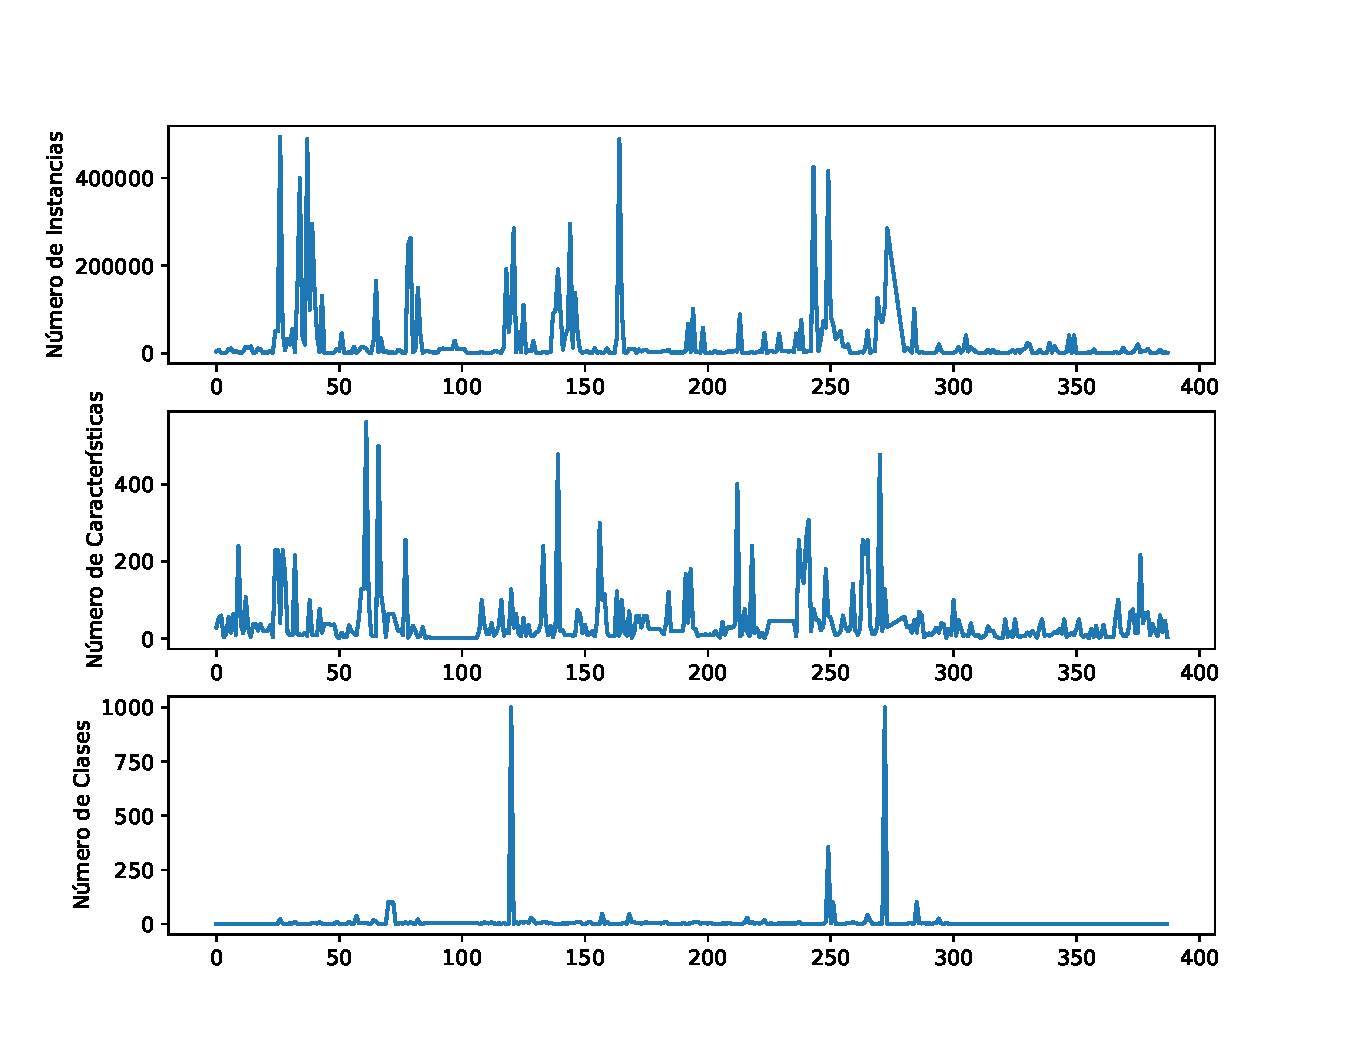
\includegraphics[scale=.75]{Figures/mtf-lineplot.pdf}
%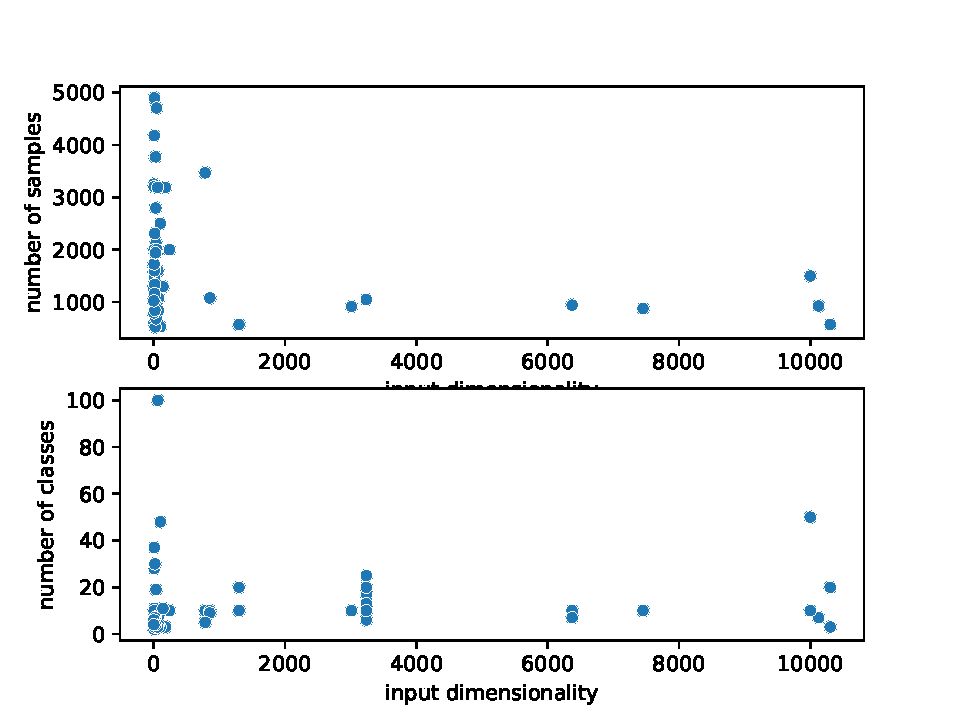
\includegraphics[scale=.60]{Figures/mtf scatterplot.pdf}
\caption{Características de los datasets en cuanto al número de instancias, número de características y número de clases.}
\label{fig:datasets}
\end{figure}
 
 
 Para la evaluación de la propuesta realizada se separaron los 388 datasets en dos conjuntos: $D_{train}$ y $D_{test}$, donde el primero representa el $80\%$ del total de datasets y el segundo el $20\%$. $D_{train}$ fue usado en el entrenamiento de las estrategias seleccionadas y $D_{test}$ en la prueba de las mismas. El conjunto de datasets de entrenamiento $D_{train}$ fue a su vez dividido en 2, usándose el segundo para la evaluación de los modelos implementados. De $D_{train}$ se usó el $75\%$ para el entrenamiento y el $25\%$ como validación, es decir, para obtener resultados parciales en cuanto al rendimiento del método implementado. En los resultados mostrados en el resto de este capítulo, se usa todo el conjunto de datasets $D_{train}$ para el entrenamiento y se exponen los resultados obtenidos en $D_{test}$.

 
 \section{Generación de Flujos}\label{sec:flujos}
 
% - Introducir la sección hablando de los tipos de algoritmos por los que está compuesto AutoGOAL (las bibliotecas que se usó, etc)
% - Hablar de cómo fue el proceso de entrenamiento de AutoGOAL para la extracción de solución, hablando de la configuración usada en AutoGOAL para la búsqueda de flujos.
% - Terminar hablando del tiempo total de entrenamiento, la cantidad total de flujos de algoritmos generados y el promedio de flujos generados por dataset.

Todos los flujos de algoritmos usados durante el entrenamiento y evaluación de la propuesta implementada fueron generadas usando AutoGOAL. Los flujos generados con AutoGOAL consisten en algoritmos que pueden encontrarse en varias bibliotecas de Python, entre las que se encuentran: Sklearn~\cite{scikit-learn}, Pytorch~\cite{paszke2019pytorch}, Keras~\cite{chollet2015keras}, NLTK~\cite{bird2009natural} y Gensim~\cite{khosrovian2008gensim}.

AutoGOAL se ejecutó en cada uno de los 388 datasets seleccionados y se guardaron todas las arquitecturas generadas junto con los resultados obtenidos. Para cada uno de los datasets, AutoGOAL se configuró para que realizara la búsqueda de flujos durante 1 hora, teniendo un total de 5 minutos para la evaluación de un flujo de algoritmos. De esta forma, se excluyeron flujos muy complejos y se garantizó la evaluación de al menos 12 flujos por dataset. Esta generación de flujos duró un total de 388 horas y se generaron en promedio 640.28 flujos de algoritmos por dataset, y en total se obtuvieron 248430  flujos. 

Estos flujos generados son usados como base de conocimiento para el método propuesto. Como se explica en la Sección~\ref{subsub:soluciones}, los flujos guardados son usados para recomendar configuraciones iniciales en el proceso de optimización en dependencia de los datasets considerados similares al dataset que se quiere evaluar.

\section{Comparación de diferentes estrategias}\label{sec:comparacion}

%- Hacer un pequeño resumen de las configuraciones de las estrategias y variantes implementadas
%
%- Hacer un resumen del resto de la sección.

Los datasets y los flujos de algoritmos extraídos fueron usados con las diferentes estrategias de meta-learning implementadas:

\begin{description}
	\item[Estrategia Vecinos más Cercanos Simple:] El ranker de vecinos cercanos, tal como está descrita en la Sección~\ref{subsub:nn}, fue probado usando la distancia L2 estándar. El ranking final que debe generar para un nuevo dataset es de 15 flujos. En esta versión se usó la estrategia simple, en la que se seleccionan \texttt{n} datasets más cercanos y de ellos los \texttt{k} flujos de algoritmos que hayan obtenido un mejor rendimiento, luego el ranking es formado seleccionando a los 15 mejores pipelines. Para la evaluación de esta estrategia se usó \texttt{k = 15} y \texttt{n = 15}.
	\item[Estrategia Vecinos más Cercanos Ponderado:] El ranker de vecinos cercanos se vuelve a probar, pero usa la otra estrategia explicada en la Sección~\ref{subsub:nn}. Esta estrategia consiste en un mecanismo ponderado entre dos factores: la distancia entre el nuevo dataset y los datasets en el conjunto de entrenamiento, y el valor del resultado del rendimiento de los flujos de algoritmos en los datasets similares. Estos factores son divididos, y el valor obtenido es el usado para generar el nuevo ranking. Al igual que en la estrategia anterior, se usa la distancia L2 estándar y se genera un ranking final de 15 flujos para una tarea nueva.
	\item[Estrategia usando  XGBRanker:] En esta estrategia, explicada en la sección~\ref{subsub:ranker}, se usó como meta-modelo XGBRanker de la biblioteca XGBoost para generar los rankings de una nueva tarea. Se usaron las siguientes configuraciones de hiperparámetros: 	
	\begin{itemize}
		\item \texttt{objective = `rank:pairwise'}: especifica la tarea de aprendizaje y el correspondiente objetivo de aprendizaje. En este caso, se eligió \textit{rank} porque es una tarea de ranking y \textit{pairwise} porque utiliza el enfoque de ranking por pares (en inglés, \textit{pairwise ranking}).
		\item \texttt{n\_estimators = 150}: Es el número de los árboles con gradientes aumentados (\textit{gradient boosted trees}) usados en el algoritmo de ranking de XGBoost explicado en la Sección~\ref{subsub:ranker}.
		\item \texttt{tree\_method = `hist'}: especifica el algoritmo de construcción de árboles usados en XGBoost~\cite{xgboost}. XGBoost dispone de 4 métodos: \texttt{exact}, \texttt{approx}, \texttt{hist}, \texttt{gpu\_hist}. El algoritmo elegido fue \texttt{hist}, que es el algoritmo más rápido, ya que es optimizado mediante un algoritmo \textit{greedy}.
		\item \texttt{max\_depth = 10}: La profundidad máxima de los árboles usados como modelos básicos. El aumento de este valor hace al modelo más complejo y más probable a sobreajustar (\textit{overfit}).
		\item \texttt{learning\_rate = 0.1}: especifica la tasa de aprendizaje.
		\item \texttt{subsample = 0.95}: proporción de la submuestra tomada de las instancias de entrenamiento. El valor 0.75 indica que XGBoost muestrearía al azar el 75\% del conjunto de entrenamiento para prevenir el sobreajuste. Esto se realiza una vez en cada iteración del algoritmo.
%		\item \texttt{colsamplebytree = 0.9}: es la proporción de submuestra de las columnas al construir cada árbol. El submuestreo ocurre una vez para cada árbol construido.
		% 		\item \texttt{random_state = 43}: Número de semilla aleatoria usado en los procesos aleatorios.
 		\item \texttt{predictor = `cpu\_predictor'}: especifica el tipo de algoritmo de predicción a usar. Los algoritmos disponibles proporcionan los mismos resultados, pero permiten el uso de la GPU o la CPU. La configuración usada fue la CPU.
	\end{itemize}
\end{description}


\subsection{Evaluación de la Precisión del Ranking}\label{subsec:ranking}

%- Explicar que se midió la precisión del ranking obtenido en las diferentes estrategias con diferentes medidas
%
%- Explicar cada una de las métricas de evaluación usadas
%
%- Explicar cómo se realizó esta experimentación
%
%- Poner resultados.

Uno de los indicadores de eficiencia de la propuesta desarrollada es la precisión del ranking obtenida en cada una de las propuestas llevadas a cabo. Para evaluar la eficacia de los modelos se compararon los rankings predichos para un determinado dataset con sus correspondientes etiquetas de ranking. Dado dos conjuntos de rankings de tamaño \texttt{k}: $T = [T_1, T_2, ..., T_k]$ y $P = [P_1, P_2, ..., P_k]$, los cuales son objetivos y predicciones respectivamente, las siguientes métricas de evaluación de ranking y funciones fueron usadas en los experimentos realizados:

\begin{description}
	\item[Coeficiente de Correlación de Rango de Spearman]o \textit{Spearman’s Rank Correlation Coefficient} (SRCC). SRCC evalúa que tan  bien puede ser descrita la relación entre el ranking verdadero y el predicho. Está definido como: $$\rho_{srccc} = 1 - \dfrac{6\sum^k_{i=1}(T_i - P_i)^2}{k(k^2-1)}$$
	
	\item[Coeficiente de Rango Ponderado]o \textit{Weighted Rank Correlation} (WRC). La métrica WRC le da más peso a los mejores candidatos. Ha sido usado en meta-learning en~\cite{sun2014MetaLearningAT, soares2004learning, costa2005weighted}. Está definido como: $$\rho_{wrc} = 1 - \dfrac{1-\sum^k_{i=1} (T_i - P_i)^2(2k - T_i - P_i + 2) }{k ^4+k^3-k^2-k}$$
	
	\item[Ganancia Acumulada Descontada Normalizada]o \textit{Normalized Discounted Cumulative Gain} (NDCG). Es una métrica de efectividad usada a menudo en motores de búsqueda usando una escala de relevancia calificada de elementos en una lista de resultados. Para entender la métrica NDGC es necesario entender primero las métricas de Ganancia Acumulada (\textit{Cumulative Gain}, CG) y Ganancia Acumulada Descontada (\textit{Discounted Cumulative Gain}, DCG).
	
	Si cada recomendación tiene una puntuación de relevancia predicha asociada con ella, CG es la suma de los valores de relevancia predichos de todos los resultados en la lista resultante. Matemáticamente, $$CG_p = \sum^k_{i=1}P_i$$
	
	El problema de CG es que no tiene en cuenta el ranking del conjunto resultante cuando determina la utilidad del conjunto. En otras palabras, si se reordenase las puntuaciones de relevancias predichas no obtendríamos un mejor conocimiento de un conjunto resultante, ya que CG no cambiará.
	
	Para superar esto se introduce DCG. DCG penaliza los documentos altamente relevantes que aparecen más abajo en la búsqueda reduciendo la relevancia predicha en dependencia de la posición del resultado. Formalmente, $$DCG_p = \sum^k_{i=1} \dfrac{2^{P_i} - 1}{log_2(i + 1)}$$
	
	Un problema surge con DCG cuando se quiere comparar el resultado de diferentes rankings porque la lista de resultados puede variar en longitud. Por lo tanto, normalizando la ganancia acumulada en cada posición se llega a NDCG. Esto se realiza ordenando los valores objetivos por su relevancia relativa, produciendo el máximo valor posible en la posición \texttt{p}. Esta última medida se denomina Ganancia Acumulada Descontada Ideal (\textit{Ideal Discounted Cumulative Gain}, IDCG), que se calcula como: $$\sum^m_{i=1} \dfrac{2^{T_i} - 1}{log_2(i+1)}, $$ donde m es la cantidad de resultados relevantes.
	Luego, NDCG se calcula como: $$NDCG_p = \frac{DCG_p}{IDCG_p}$$
\end{description}

La siguiente figura muestra los resultados obtenidos en cada una de las estrategias explicadas en la Sección~\ref{sec:comparacion}.

[hablar un poco de los que se ve en las gráficas]

\subsection{Resultados Experimentales}\label{subsec:resultados}

%- Explicar cómo se realizaron los experimentos.
%
%- Hablar de los diferentes aspectos evaluados (flujos inválidos, mejor resultado, iteraciones para el mejor resultado...).
%
%- Exponer los resultados.

La eficacia del método implementado no se basa solo en qué tan bueno es para la creación de rankings  de flujos de algoritmos basados en experiencias pasadas. Para la evaluación del método es importante conocer los resultados obtenidos al incorporarse a un sistema de AutoML. Es decir, cómo el ranking de configuraciones elegidas son usadas para inicializar el proceso de optimización, y qué resultados este proceso puede obtener al usar el conocimiento previo adquirido mediante meta-learning. En esta sección se discuten las experimentaciones realizadas para evaluar estos aspectos.

Para la realización de las experimentaciones se ejecutó la búsqueda algoritmos de AutoGOAL con y sin meta-learning, probando los tres métodos de meta-learning mencionados anteriormente: vecinos cercanos con la estrategia simple, vecinos cercanos usando mecanismos ponderados y usando un ranker. Para estudiar su rendimiento bajo una estricta restricción de tiempo, y además, debido a limitaciones de los recursos computacionales usados, se limitó la búsqueda para cada ejecución a 30 minutos. Igualmente, el tiempo de ejecución de un solo modelo se limitó a la sexta parte de este tiempo (5 minutos). Las evaluaciones realizadas en esta sección muestran los resultados obtenidos en los datasets de prueba, usando los datasets de entrenamiento para entrenar los métodos implementados. Cada estrategia se ejecutó 3 veces, y los resultados mostrados son el promedio de estas ejecuciones. 

Uno de los aspectos a analizar es la cantidad de flujos de algoritmos inválidos generados durante el proceso de optimización. Los flujos inválidos se encuentran en dos casos: cuando se excede el tiempo de espera predefinido por el investigador, o cuando ocurren errores de tiempo de ejecución impredecibles, como errores de falta de memoria provocados por una combinación inviable de hiperparámetros. Estas circunstancias a menudo son imposibles de predecir de antemano y, como tal, no se pueden tener en cuenta en las gramáticas de AutoGOAL. Sin embargo, mediante la información adquirida con meta-learning se espera que la cantidad de flujos inválidos disminuya, ya que se utiliza conocimiento adquirido de problemas similares que usan flujos de algoritmos válidos. En la Figura \ref{fig:failedpipelines}, se muestran los resultados obtenidos usando cada una de las estrategias desarrolladas, incluyendo la versión de AutoGOAL que no utiliza la inicialización de meta-learning.

\begin{figure}[H]
\centering
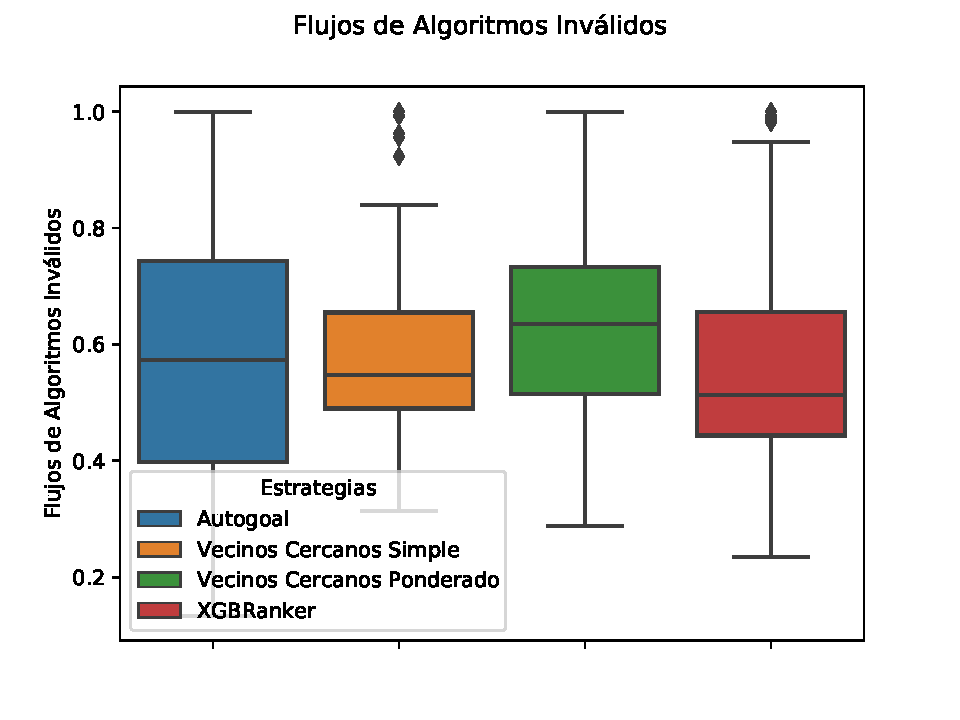
\includegraphics[scale=.75]{Figures/failed-pipelines.pdf}
\caption{Cantidad de flujos de algoritmos inválidos generados en cada uno datasets usando las diferentes estrategias.}
\label{fig:failedpipelines}
\end{figure}

%Otro de los aspectos que puede ser interesante evaluar son las iteraciones necesarias para la obtención del mejor resultado. La Figura \ref{fig:maxidx} muestra los resultados obtenidos a través de las iteraciones en las diferentes versiones evaluadas. Se puede observar que las dos estrategias de vecinos cercanos obtuvieron el mejor resultado en menos iteraciones que AutoGOAL sin meta-learning. Sin embargo, la estrategia de XGBRanker no obtuvo el mismo resultado. % El resultado más sorprendente es que meta-learning produjo mejoras drásticas a partir de la primera configuración que seleccionó y que se prolongó hasta el final del experimento. La mejora fue más pronunciada al principio y, con el tiempo, AutoGOAL sin meta-learning también encontró buenas soluciones, lo que le permitió alcanzar los mismos resultados obtenidos en las versiones que usan meta-learning en algunos datasets (mejorando así su clasificación general).
%
%\begin{figure}[H]
%\centering
%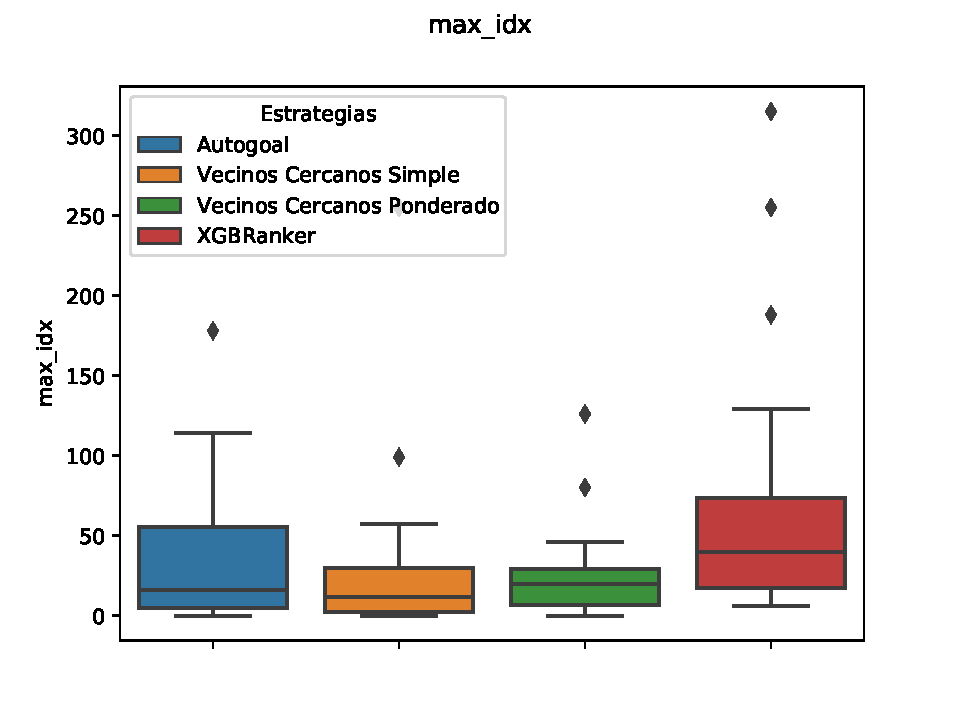
\includegraphics[scale=.60]{Figures/max idx.pdf}
%\label{fig:maxidx}
%\caption{Cantidad de iteraciones necesarias para la obtención del mejor resultado promedio en cada uno datasets usando las diferentes estrategias.}
%\end{figure}

Otro de los aspectos que puede ser interesante de evaluar es el comportamiento de las soluciones obtenidas a través de distintas las distintas iteraciones de AutoGOAL. La Figura~\ref{fig:performance} muestra la media y el intervalo de confianza del 95\% obtenido a través de las iteraciones en las diferentes estrategias evaluadas. Se puede observar como, a partir de determinado punto (cuando se terminan las iteraciones iniciales que generan resultados aleatorios) las soluciones que usan meta-learning alcanzan mejores resultados. En la mayor parte del tiempo estos resultados se mantienen, por lo que las soluciones de meta-learning superan a las soluciones obtenidas mediante AutoGOAL sin el uso de meta-learning.

\begin{figure}[H]
\centering
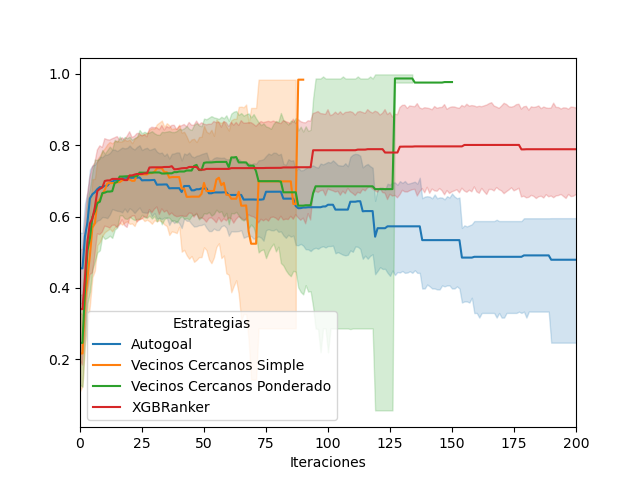
\includegraphics[scale=.75]{Figures/performance}
\caption{Resultados de rendimiento obtenidos en los datasets de prueba, se muestra la media y el intervalo de confianza del 95\%.}
\label{fig:performance}
\end{figure}

En la Figura \ref{fig:bestfn} se muestra el mejor resultado final obtenido en la búsqueda de los flujos de algoritmos en cada uno de los datasets de prueba para las diferentes estrategias. Como se puede apreciar, se obtienen mejores resultados finales en cada uno de las estrategias seguidas con respecto a AutoGOAL sin meta-learning. La diferencia entre la estrategia de vecinos cercanos simple no es tan pronunciada con respecto a  la versión que no usa meta-learning, y esto se cree que se debe a que, a pesar de que mediante esta estrategia se obtienen los valores óptimos más rápidos, AutoGOAL es capaz de alcanzar a esta versión, y encontrar buenas soluciones. El método de vecinos cercanos ponderado y el que usa XGBRanker, un algoritmo de ranking de XGBoost, sí obtiene resultados un poco más significativos, siendo este último el que mejor resultado final obtiene.

\begin{figure}[H]
\centering
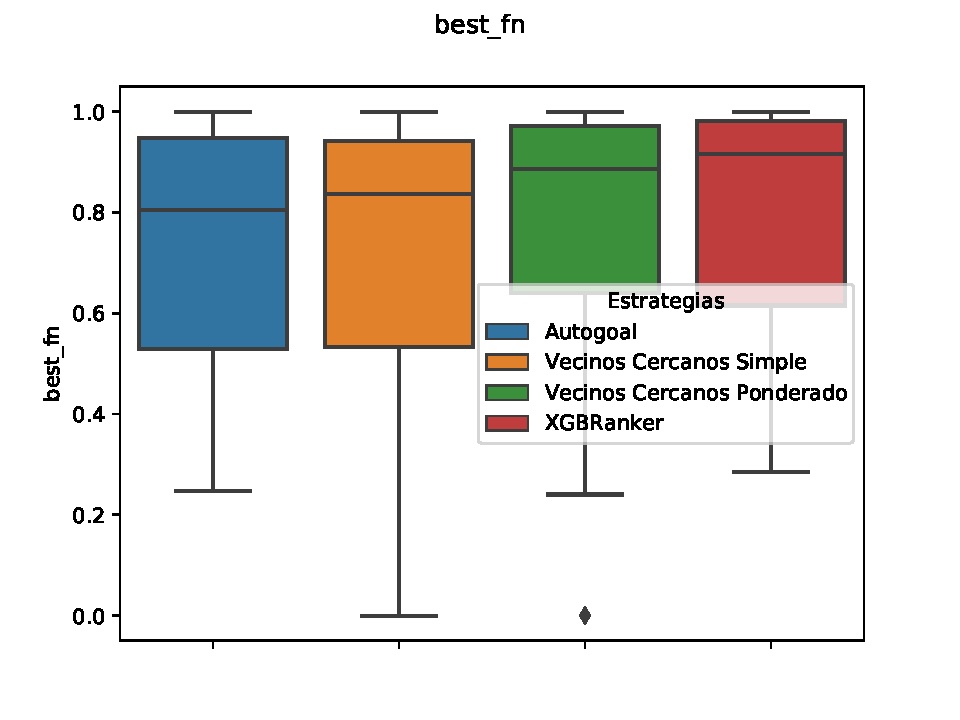
\includegraphics[scale=.75]{Figures/best-fn.pdf}
\caption{Mejor resultado obtenido en la búsqueda de los flujos de algoritmos en cada uno de los datasets de prueba para las diferentes estrategias.}
\label{fig:bestfn}
\end{figure}

\section{Discusión}\label{sec:discusion}

%- Hablar de la evidencia de que el sistema funciona 
%
%- Limitaciones:
%
%	+ Tener en cuenta métricas multi-objetivos
%	
%	+ Adaptarlo para usar regresión
%	
%	+ Hablar de las limitaciones de los datasets, de mayor variedad y de una mayor diversificación en sus características
%	
%	+ Hablar de los meta-features, del estudio la posible selección de estas

En cuanto a los resultados experimentales, es importante tener en cuenta que estos se implementan utilizando el mismo código en todos los experimentos, variando solo la definición de los tipos de entrada y salida. Para cada una de las variantes analizadas, los experimentos se ejecutan bajo la misma restricción de tiempo (30 minutos de ejecución total y 5 minutos de ejecución para un solo modelo), por lo tanto, cada una de las variantes probadas tiene el mismo tiempo para la búsqueda de los flujos de algoritmos. Las experimentaciones realizadas muestran que el conocimiento adicional obtenido al principio mediante la técnica de meta-learning desarrollada cuando es agregado al proceso de optimización, obtiene resultados satisfactorios. En cuanto a la cantidad de flujos inválidos generados y la velocidad con la que se encuentra el mejor resultado de rendimiento, en promedio, los modelos que usan la técnica de meta-learning obtienen mejores resultados con respecto al modelo donde no se aplica.

Por otro lado, también se obtiene un buen rendimiento al usar el sistema de recomendación de meta-learning para predecir flujos de algoritmos por sí solos. Es decir, sin añadir un extenso proceso de optimización posteriormente. Estas afirmaciones se pueden demostrar mediante los buenos resultados obtenidos para la predicción de rankings realizados.

La estrategia de ranking más usada en la literatura~\cite{fuerer2015efficient, sun2014MetaLearningAT, bradzil2009metalearning} se basa en \textit{average ranking} o ranking promedio~\cite{bradzil2009metalearning}. Sea $R_{i,j}$ el ranking del algoritmo $T_{j}$, $j=1,...,t$ en el dataset $i$, donde $t$ es el número de algoritmos, el ranking promedio de cada algoritmo $T_{j}$ está definido como: $\overline{R_{j}} = \sum^{k}_{i=1}R_{i,j} / k$, donde $k$ es el número de datasets similares. Es decir, el ranking promedio de un algoritmo no es más que el promedio del ranking obtenido en cada uno de los datasets seleccionados. El ranking final es calculado ordenando los ranking promedio de todos los algoritmos. Una de las razones por la que esta estrategia no fue usada, es que este método de agregación de rankings requiere la evaluación de cada flujo de algoritmos en todos los datasets, por lo que la agregación de un nuevo dataset en la base de conocimiento requiere la evaluación de todos los flujos de algoritmos anteriores en el dataset. Usualmente se implementa mediante la selección de un conjunto predefinido de flujos de algoritmos, por lo que no existe mucha variedad en los flujos utilizados para la inicialización de los proceso de optimización. La estrategia de generación de ranking seguida por la implementación del método de vecinos cercanos proporciona una forma fácil de agregar nuevos datasets a la base de conocimiento usada, y una mayor variedad en los flujos de algoritmos utilizados.

El método propuesto tiene también algunas limitaciones, las cuales se pueden mejorar en trabajos futuros. Con respecto a la métrica usada para determinar el rendimiento de cada flujo, se usa la métrica por defecto de AutoGOAL, \textit{accuracy}. Sin embargo, en escenarios prácticos, puede ser necesario equilibrar diferentes métricas de rendimiento, incluido también el uso del tiempo y la memoria, y cualidades más subjetivas como la interpretabilidad de los modelos o su capacidad para lidiar con datos sesgados. El enfoque de optimizar una métrica principal sujeta a restricciones de tiempo y memoria usada en AutoGOAL, y por lo tanto también en nuestra propuesta, es insuficiente en un escenario en el que el usuario final tiene que decidir sobre cuestiones prácticas como el despliegue de estos flujos en un sistema de producción. A modo de ejemplo, TPOT~\cite{olson2019tpot} considera este problema desde el enfoque multi-objetivo mediante la optimización conjunta de la precisión y la complejidad del modelo (en términos de longitud de los flujos). También se han implementado eficientemente medidas multi-criterio en sistemas de meta-learning~\cite{bradzil2003ranking}, donde se crea el ranking de algoritmos basado en \textit{accuracy} y tiempo, mediante la métrica denominada \textit{Adjusted Ratio of Ratios} (ARR)~\cite{soares2000measures}

Los experimentación llevada a cabo se realizó solo con datasets de clasificación, por lo que solo se estudiaron los resultados obtenidos en esa tarea. Sin embargo, el modelo propuesto es adaptable a cualquier tipo de problema de aprendizaje de máquinas siempre y cuando se tenga una medida para determinar la eficiencia de un flujo de algoritmos en un dataset. Para la realización de varios tipos de tareas, se propone la creación de un modelo diferente para cada tipo de problemas. Es decir, se crearía un modelo para las tareas de clasificación y otro para regresión. De esta manera, para el análisis de un dataset es necesario conocer el tipo de tarea que se quiere resolver, y usar el modelo adecuado para ella.

Meta-learning es muy dependiente de la calidad de los meta-ejemplos que usa para su entrenamiento~\cite{gomes2012combining}. Usualmente es difícil obtener buenos resultados ya que las meta-características son en general bastante ruidosas y el número de problemas disponibles para la generación de meta-ejemplos usualmente es limitada. En este trabajo, se obtienen buenos resultados debido al uso de meta-características que han sido ampliamente usadas en la literatura y a la gran variedad de datasets extraídos. Sin embargo, se cree que un análisis más detallado de la distribución de los datasets y la inclusión de datasets de mayor tamaño puede proporcionar mejores resultados. De igual manera, un estudio de las meta-características para la eliminación de aquellas que proporcionen información poco útil puede proporcionar mejoras en el método propuesto.

La generación de rankings en la estrategia de vecinos cercanos es otro de los aspectos que necesita ser estudiado más detalladamente. El método de generación de ranking mediante el mecanismo ponderado, en el que se tiene en cuenta la distancia entre el dataset a analizar y los datasets de la base de conocimiento y el valor del rendimiento de un flujo de algoritmos, puede ser mejorado. En la versión utilizada, se le da la misma importancia a ambos factores, quizá dándole más peso a uno de los dos componentes mejoren los resultados obtenidos. De esta forma, para la generación de rankings, por ejemplo, los resultados de rendimiento de los flujos de algoritmos pueden considerarse más importantes, priorizando este factor en el ranking resultante.






